\documentclass[10pt,twocolumn,a4paper]{article}
\usepackage[utf8]{inputenc}
\usepackage[T1]{fontenc}
\usepackage{mathptmx}
\usepackage{microtype}
\usepackage[margin=1.8cm,columnsep=0.7cm]{geometry}
\usepackage{amsmath,amssymb}
\usepackage{graphicx}
\usepackage[hidelinks]{hyperref}
\usepackage{xcolor}
\usepackage{titlesec}
\usepackage{enumitem}
\usepackage[font=small,labelfont=bf]{caption}
\usepackage{abstract}

\titleformat{\section}{\normalfont\large\bfseries}{\thesection}{0.6em}{}
\titleformat{\subsection}{\normalfont\normalsize\bfseries}{\thesubsection}{0.6em}{}
\titlespacing*{\section}{0pt}{1.1em}{0.4em}
\titlespacing*{\subsection}{0pt}{0.8em}{0.3em}
\setlist{itemsep=1pt,topsep=3pt,leftmargin=1.3em}
\renewcommand{\abstractnamefont}{\normalfont\bfseries}
\renewcommand{\abstracttextfont}{\normalfont\small}
\newcommand{\ab}{\bar\alpha}

\title{\Large\bfseries From Noise to Boundaries:\\Area-Law Information Scaling Along the Diffusion Path}
\author{St\'ephane Cuenat\\[2pt]
\small Independent researcher \quad\texttt{stephane.cuenat@gmail.com}\\[1pt]
\small\textit{Preprint draft, 16 October 2026. Pilot results computed on CPU only.}}
\date{}

\begin{document}
\twocolumn[
\begin{@twocolumnfalse}
\maketitle
\vspace{-1.5em}
\begin{abstract}
\noindent The holographic principle holds that the information in a region of space scales with its boundary area, not its volume. We ask whether a similar law governs structure that emerges from maximal disorder in generative AI. Diffusion models build images from pure Gaussian noise, a maximum-entropy state, and for Gaussian-mixture data models every marginal along the generation path is exact. We measure how the mutual information between an image region and its complement scales with region size, comparing each model against a Gaussian control with identical covariance.
On a learned model of real handwritten digits (MNIST, $28{\times}28$), finished images obey an area law (scaling exponent $\beta = 1.07$ over regions of 2--12 pixels). Along the generation path, non-Gaussian structure contributes up to $2.4\times$ the control's information; this excess scales in a bulk-like way in the noisy phase (exponent 1.68) and shifts smoothly toward boundary scaling as details form (1.17), with no sharp transition at our resolution. A synthetic experiment isolates the mechanism: global structure, once decided, carries size-independent information. The picture that emerges is that \emph{structure is decided in the bulk and written on the boundary}.
All results were obtained on two CPU cores in under 30 minutes. We outline how the same measurement can serve as a diagnostic for generative models and as a concrete, testable counterpart to holographic ideas.
\end{abstract}
\vspace{1.2em}
\end{@twocolumnfalse}
]

\section{Introduction}
In physics, how information is spread across space is a deep diagnostic of structure. The holographic principle states that the maximum information in a region scales with its boundary area, not its volume; the Bekenstein--Hawking entropy of a black hole is the canonical case~\cite{bekenstein}. Ground states of local quantum systems obey the same \emph{area law} for entanglement, while generic random states obey a \emph{volume law}.

Recent work pushes this further. Miyashita, Sekino and Susskind argue that an entire toy standard model can emerge holographically from a system at infinite temperature, a maximum-entropy state with no preferred structure~\cite{mss}. This raises a general question: \textbf{when structure emerges from maximal disorder, does its information organize on boundaries?}

Diffusion generative models provide a uniquely controllable laboratory for this question. They begin from isotropic Gaussian noise, also a maximum-entropy state, and progressively build structured images. Unlike cosmology, every intermediate state is observable, the process can be rerun at will, and for suitable data models every marginal along the generation path is known in closed form.

We ask whether the mutual information between an image region and its complement scales with the region's perimeter (area law) or its size (volume law), and how this changes along the path from noise to image.

\paragraph{Contributions.}
\begin{enumerate}
\item An exact framework: for Gaussian-mixture data, diffusion marginals stay Gaussian mixtures, so region--complement mutual information can be computed with exact densities and a same-covariance Gaussian control that isolates non-Gaussian structure.
\item Evidence that finished images of real handwritten digits obey an area law ($\beta \approx 1.07$ over a $6\times$ range of region sizes).
\item A new signature along the generation path: in the noisy phase, non-Gaussian structure carries extra information with \emph{bulk-like} scaling that transfers to the boundary as details are formed.
\item A fully CPU-only, reproducible pipeline, showing that this line of work does not require large compute to begin.
\end{enumerate}

\section{Related work}
\paragraph{Holography and deep networks.} Hashimoto et al.\ represented AdS/CFT as a deep network whose depth plays the role of the emergent radial dimension~\cite{hashimoto}. Mehta and Schwab mapped deep networks onto renormalization-group flow~\cite{mehta}. Both treat network architecture as geometry; we instead measure the \emph{information geometry of generated data}.

\paragraph{Information and area laws in data.} Cheng, Chen and Wang estimated mutual information in MNIST and found it far below its upper bound, suggesting a shared inductive bias toward low information complexity~\cite{cheng}. Locally connected neural-network quantum states are known to obey an entanglement area law~\cite{arealawnn}. We are not aware of work measuring how region--complement information scales \emph{along} a generative trajectory.

\paragraph{Phase transitions in diffusion.} Biroli et al.\ identify three regimes in the backward diffusion process, separated by speciation and collapse crossovers~\cite{biroli}. Sclocchi, Favero and Wyart show a phase transition at which high-level features such as class are decided~\cite{sclocchi1}, and that changes during forward--backward experiments occur in correlated chunks whose length scale diverges at that transition~\cite{sclocchi2}. Our noisy-phase bulk-like signal is a natural information-theoretic counterpart to this picture.

\section{Framework}
\paragraph{Exact diffusion marginals.} Consider data modelled as a Gaussian mixture with weights $w_k$, means $\mu_k$ and covariances $\Sigma_k$. Under the variance-preserving forward process with signal fraction $\ab\in[0,1]$, the marginal stays a Gaussian mixture:
\begin{equation}
p_{\ab}(x)=\sum_k w_k\,\mathcal N\!\left(x;\ \sqrt{\ab}\,\mu_k,\ \ab\,\Sigma_k+(1-\ab)I\right).
\end{equation}
A perfectly trained reverse process has the same marginals, so this describes the generation path of an ideal diffusion model of the learned density, from pure noise ($\ab=0$) to data ($\ab=1$).

\paragraph{Region--complement information.} For a centred $L\times L$ region $A$ and its complement $B$ we compute
\begin{equation}
I(A;B)=\mathbb E_{x\sim p_{\ab}}\!\left[\log p_{\ab}(x)-\log p_{\ab}(x_A)-\log p_{\ab}(x_B)\right]
\end{equation}
by Monte Carlo with exact densities, since marginals of a Gaussian mixture on any pixel subset are again Gaussian mixtures. No learned estimator is involved; the only error is sampling error, reported for every value.

\paragraph{Gaussian control.} For each $\ab$ we compare with a single Gaussian having exactly the same covariance. Its information is exact (log-determinants). Any difference between model and control is therefore due to non-Gaussian structure, not to second-order correlations.

\paragraph{Scaling exponent.} We fit $I(L)\propto L^{\beta}$ on log--log axes. For 2D images, $\beta=1$ is an area (perimeter) law and $\beta=2$ a volume law. We also report the excess $I_{\text{model}}-I_{\text{control}}$ and its own exponent.

\paragraph{Settings.} Three data models of increasing realism: (i) a Gaussian random field with a natural-image-like $1/k^2$ spectrum on a $40\times40$ torus; (ii) a synthetic 16-class mixture of smooth global patterns plus local texture ($24\times24$); (iii) a learned 40-component full-covariance mixture of MNIST ($28\times28$, four $k$-means sub-clusters per digit), selected on held-out likelihood, where it beats the single Gaussian by about 207 nats per image.

\section{Results}
\subsection{Validation and Gaussian baseline}
The framework behaves as required on fields with known answers. White noise gives zero information. Short-range and $1/k^2$ fields give $\beta=1.01$ and $1.03$, and strips that grow in area at fixed boundary length give constant information, confirming that the measure tracks boundaries rather than volume.

Along the generation path of a natural-like Gaussian field, the area law emerges smoothly: $\beta$ drifts from 1.40 near pure noise to 1.03 at the end, with no transition (Fig.~\ref{fig:gauss}). Gaussian data cannot produce a phase transition, so this serves as the null baseline.

\begin{figure}[t]
\centering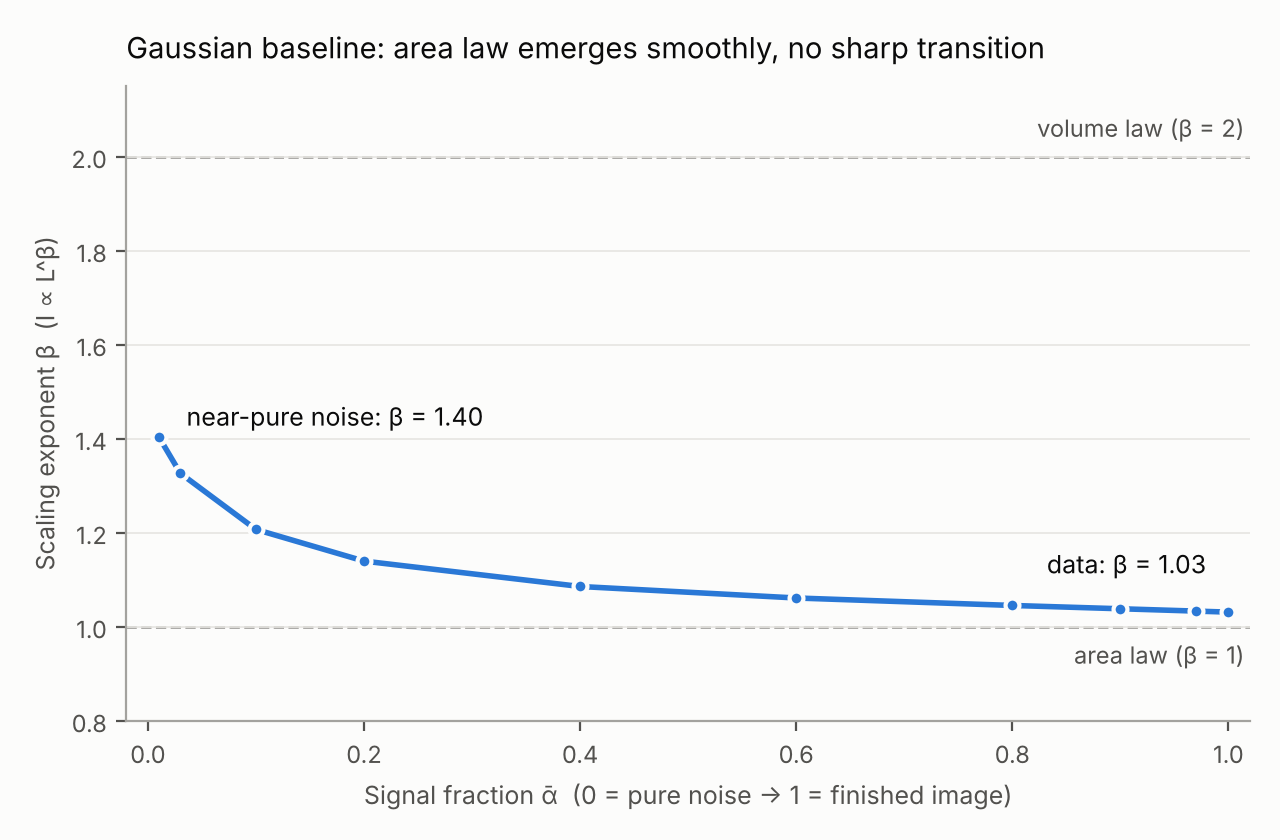
\includegraphics[width=\columnwidth]{beta_trajectory.png}
\caption{Gaussian baseline: scaling exponent along the generation path of a $1/k^2$ random field.}
\label{fig:gauss}
\end{figure}

\subsection{Synthetic non-Gaussian data}
For a 16-class mixture of smooth global patterns, the model and its same-covariance control coincide ($\beta\approx1.8$--$1.9$) while the class is being decided ($\ab\approx0.002$--$0.04$). Once the class is fixed, the mixture leaves the Gaussian path: $\beta$ falls through the area law to about 0.4, because the dominant shared information is a single global fact ($\log 16\approx2.8$ nats) that every region already carries (Fig.~\ref{fig:mix}). The control declines only to 1.2 and ends with five times more information.

This isolates a mechanism: discrete global structure, once decided, contributes size-independent information, reminiscent of the constant term in topological entanglement entropy.

\begin{figure}[t]
\centering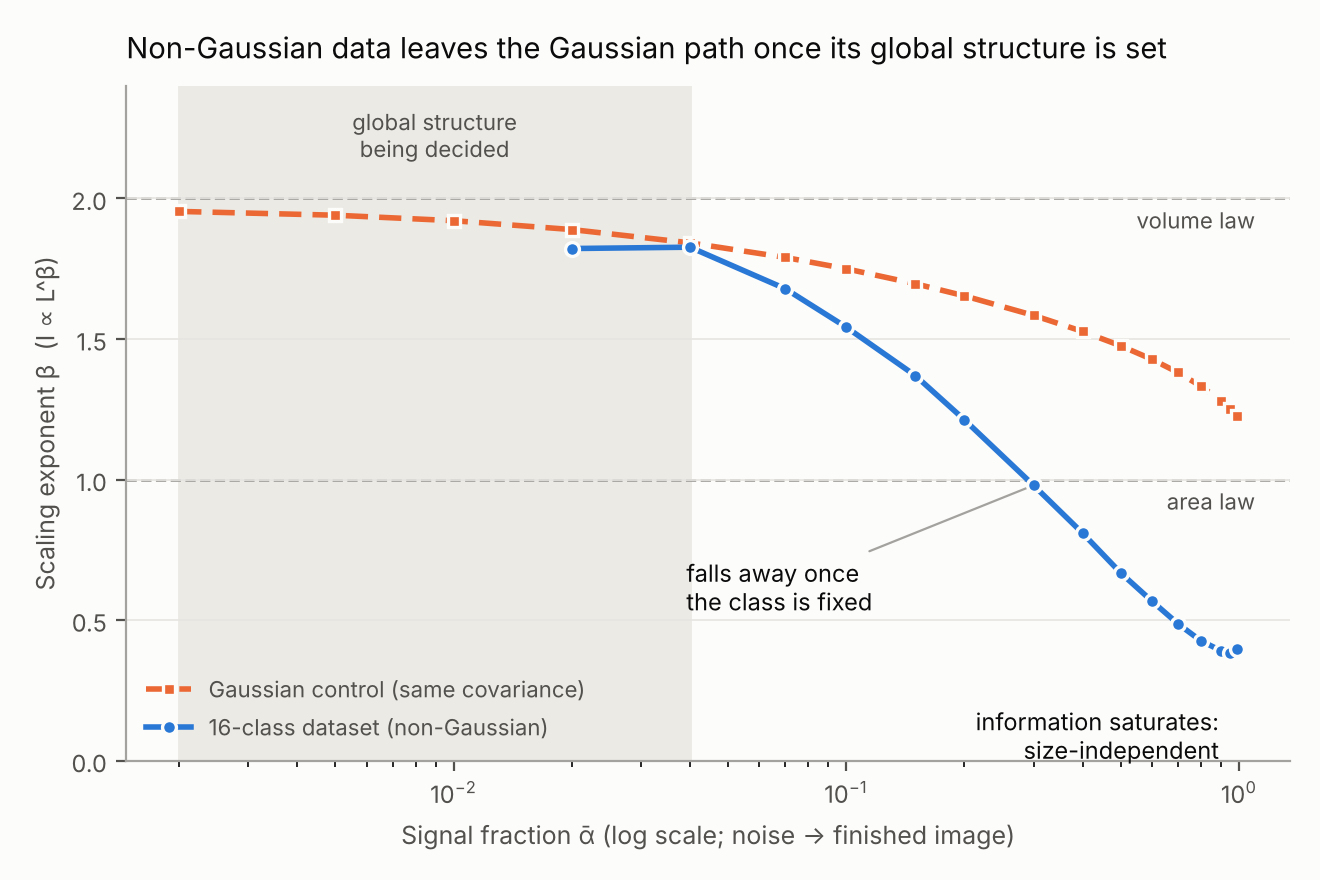
\includegraphics[width=\columnwidth]{beta_mixture_vs_control.png}
\caption{Synthetic 16-class data vs.\ Gaussian control. Shaded: window in which the class is decided.}
\label{fig:mix}
\end{figure}

\begin{figure*}[t]
\centering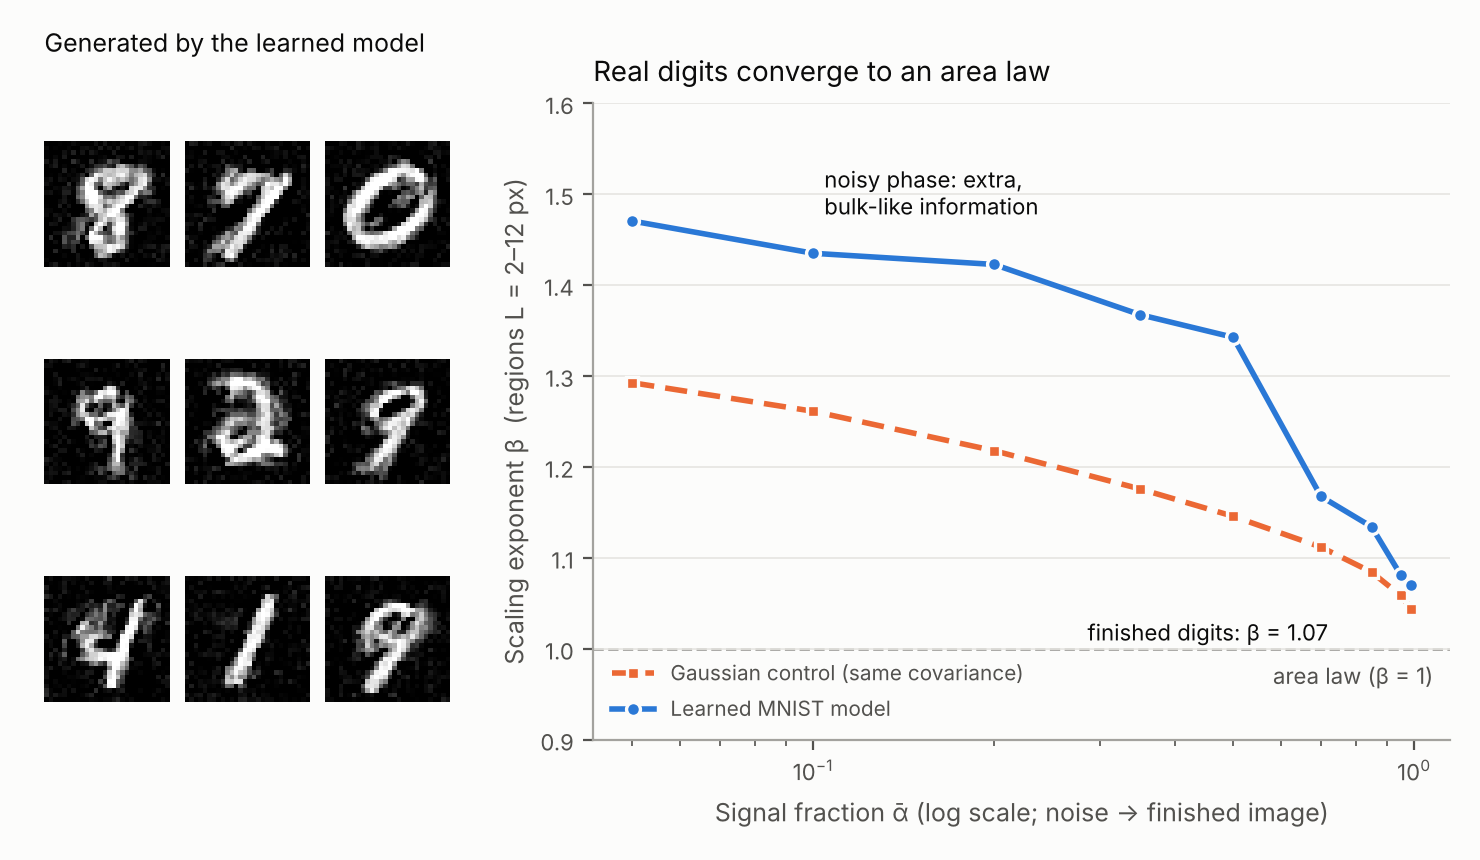
\includegraphics[width=0.82\textwidth]{mnist_beta.png}
\caption{Learned MNIST model vs.\ Gaussian control along the generation path. Left: samples drawn from the learned model.}
\label{fig:mnist}
\end{figure*}

\subsection{Learned model of MNIST}
On real $28\times28$ digits, finished images obey an area law: $\beta=1.07$ over regions of 2--12 pixels (control 1.04). Along the path, the learned model sits well above the control in the noisy phase ($\beta\approx1.43$--$1.47$ vs.\ 1.26--1.29 at $\ab\le0.2$) and converges as details form (Fig.~\ref{fig:mnist}).

The excess information $I_{\text{model}}-I_{\text{control}}$ scales with exponent 1.6--1.7 in the noisy phase, bulk-like, and 1.1--1.3 near the end, boundary-like. The model-to-control ratio peaks at $2.4\times$ around $\ab\approx0.1$--$0.2$ and settles at about $1.35\times$. Regions larger than $L\approx14$ are excluded from fits because their complement is mostly blank border; Monte Carlo errors are at most 0.14 nats.

\subsection{Is the transition sharp?}
A coarse grid suggested a steep change between $\ab=0.5$ and $0.7$. We repeated the measurement on 11 noise levels between 0.3 and 0.9 with three independent seeds, each refitting the model and redrawing all Monte Carlo samples.

The change is \textbf{smooth} (Fig.~\ref{fig:fine}). The model's $\beta$ declines monotonically from $1.41\pm0.01$ to $1.10\pm0.003$, by about 0.03--0.04 per step, with no jump larger than the seed-to-seed spread. The apparent steep drop on the coarse grid was within single-run noise. The exponent of the non-Gaussian excess falls just as smoothly, from $1.68\pm0.02$ (between area and volume law) to $1.17\pm0.02$ (near area law).

At this resolution and model class, the hypothesis of a sharp transition is therefore not supported: the bulk-to-boundary shift is a crossover, not a phase transition.

\begin{figure*}[t]
\centering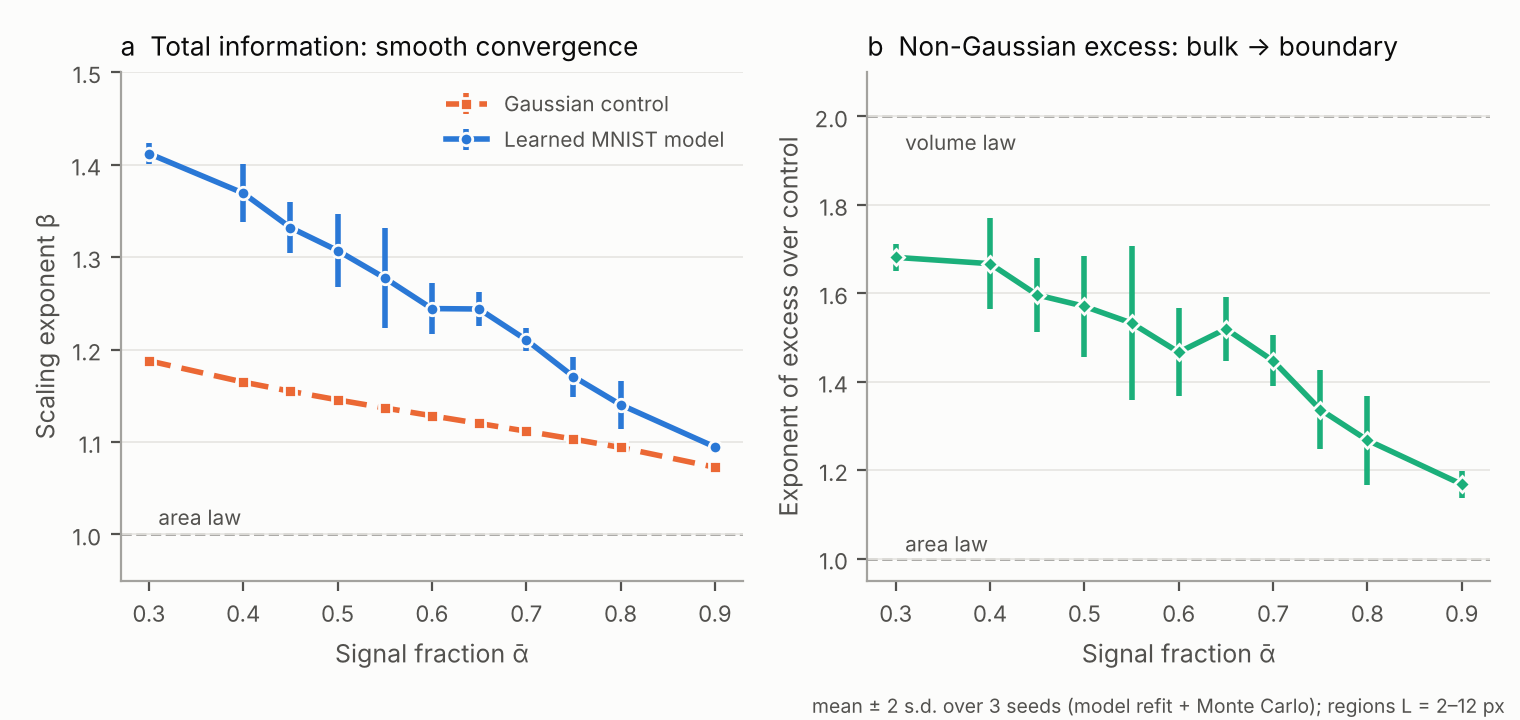
\includegraphics[width=0.86\textwidth]{mnist_fine.png}
\caption{Fine-grid test. (a) Scaling exponent of total information, model vs.\ control. (b) Exponent of the model's excess over the control. Mean $\pm$ 2 s.d.\ over 3 seeds.}
\label{fig:fine}
\end{figure*}

\section{Discussion}
\paragraph{Interpretation.} Across all three settings a consistent picture emerges. Generation begins from a state with no information. In the noisy phase, the coarse, global properties of the image (which digit, its overall layout) are decided, and the information they carry scales with region \emph{size}: every pixel contributes evidence about a shared global fact. As details form, information becomes increasingly local and settles onto region \emph{boundaries}. Finished real images obey an area law. In short: structure is decided in the bulk and written on the boundary.

\paragraph{Potential.} If the picture holds for trained neural networks and natural images, it opens several directions:
\begin{itemize}
\item \textbf{A diagnostic for generative models.} The scaling exponent and the excess over a Gaussian control are cheap, interpretable numbers that summarize how a model organizes information, complementing sample-quality metrics. Departures from the expected profile could flag memorization or missing global structure.
\item \textbf{Better sampling schedules.} The bulk-to-boundary crossover marks where global decisions end and local refinement begins, suggesting where to concentrate denoising steps.
\item \textbf{Architecture design.} Area-law data suit models with locality priors; the bulk-like noisy phase suggests where global attention matters most. This is directly testable by comparing U-Net and transformer denoisers.
\item \textbf{A bridge to physics.} Area laws are the signature of holographic organization. Finding them emerge from noise in learned systems, with no gravity involved, suggests boundary-organized information may be a general property of structure formation rather than a peculiarity of black holes. This is an analogy to be tested, not a claim about the universe, but it gives the holographic intuition a concrete, measurable counterpart.
\item \textbf{Accessible science.} The entire pilot ran on two CPU cores in under 30 minutes. Careful controls and exact computations, not scale, carried the result.
\end{itemize}

\paragraph{Limitations.} The learned model is a 40-component Gaussian mixture, not a neural network; trained denoisers may organize information differently. Images are small ($28\times28$) and region fits span $L=2$--$12$, less than a decade, with edge effects beyond. The synthetic results depend on the balance between global and local structure. A sharp transition was not supported; sharp transitions may still appear in richer, hierarchical data or larger dimensions, where diffusion phase transitions are predicted to sharpen.

\section{Roadmap and reproducibility}
The pilot was designed so each step can run on modest hardware. The path to a full paper:
\begin{enumerate}
\item \textbf{Trained neural denoisers.} Repeat the measurement with small U-Net and transformer (DiT) diffusion models trained on MNIST and CIFAR-10, using the exact-mixture results here as a calibrated reference. Tests whether the scaling depends on architecture. Laptop CPU for MNIST; a single GPU for CIFAR-10.
\item \textbf{Learned estimators, validated.} For trained networks exact densities are unavailable; validate $k$-NN and neural mutual-information estimators against the exact values from this pilot before use.
\item \textbf{Larger images and a full decade of scales.} Natural images at $64\times64$ or more, with periodic or padded regions to remove edge effects.
\item \textbf{Link to diffusion phase transitions.} Compare the location of the bulk-to-boundary shift with speciation times computed from the data covariance spectrum~\cite{biroli}.
\item \textbf{Theory.} Derive the excess-information exponent for mixture models analytically, starting from the class-information decomposition used in the synthetic experiment.
\end{enumerate}

\paragraph{Reproducibility.} All experiments use NumPy, SciPy and scikit-learn on 2 CPU cores; total compute for all results in this draft is under 30 minutes. Scripts and result files will be released with the preprint.

\small
\begin{thebibliography}{10}\setlength{\itemsep}{1pt}
\bibitem{mss} S.~Miyashita, Y.~Sekino, L.~Susskind, \href{https://arxiv.org/abs/2607.05678}{Holograms and Standard Models}, arXiv:2607.05678 (2026).
\bibitem{hashimoto} K.~Hashimoto, S.~Sugishita, A.~Tanaka, A.~Tomiya, \href{https://arxiv.org/abs/1802.08313}{Deep learning and AdS/CFT}, Phys.\ Rev.\ D 98, 046019 (2018).
\bibitem{mehta} P.~Mehta, D.~J.~Schwab, An exact mapping between the variational renormalization group and deep learning, arXiv:1410.3831 (2014).
\bibitem{cheng} S.~Cheng, J.~Chen, L.~Wang, \href{https://arxiv.org/abs/1712.04144}{Information perspective to probabilistic modeling: Boltzmann machines versus Born machines}, Entropy 20, 583 (2018).
\bibitem{arealawnn} \href{https://arxiv.org/abs/1907.11333}{Entanglement area law for shallow and deep quantum neural network states}, arXiv:1907.11333 (2019).
\bibitem{biroli} G.~Biroli, T.~Bonnaire, V.~de~Bortoli, M.~M\'ezard, \href{https://arxiv.org/abs/2402.18491}{Dynamical regimes of diffusion models}, Nature Communications 15 (2024).
\bibitem{sclocchi1} A.~Sclocchi, A.~Favero, M.~Wyart, \href{https://arxiv.org/abs/2402.16991}{A phase transition in diffusion models reveals the hierarchical nature of data}, PNAS (2025).
\bibitem{sclocchi2} A.~Sclocchi, A.~Favero, N.~I.~Levi, M.~Wyart, Probing the latent hierarchical structure of data via diffusion models, ICLR (2025).
\bibitem{bekenstein} J.~D.~Bekenstein, Black holes and entropy, Phys.\ Rev.\ D 7, 2333 (1973).
\bibitem{cuenat} S.~Cuenat, L.~Andr\'eoli, A.~N.~Andr\'e, P.~Sandoz, G.~J.~Laurent, R.~Couturier, M.~Jacquot, Fast autofocusing using tiny transformer networks for digital holographic microscopy, Optics Express 30(14) (2022).
\end{thebibliography}
\end{document}
